% \section*{Results - network model}
% \subsection*{The integrate- and fire best fit}
% Table (\ref{table:integrate-and-fire_parameters}) show the best fit parameters to the integrate-and-fire model for different percentages of the two mutated channels. The mean absolute difference between the NEURON and the integrate-and-fire current-frequency curves was used as it yielded a better fit than the root mean square. The refractory period was set to 5 ms to avoid overfitting.

% \begin{table}
%  \centering
%  \caption{The parameters found by the best fit of the basic integrate-and-fire model to the NEURON data. Error is the mean of the absolute difference between the NEURON frequency-current graph and the integrate-and-fire one. $t_r=$5 ms.}
%  \begin{tabular}{r|c|r|r|r|r|r} 
%   Mut. & Unmut. ch. & $\tau$ & $V_{thr}$ & $V_{r}$ & $R$ & Error\\
%   \hline
%   Q1481K & 100 \% & 43.6 & 20.1 & -98.2 & 66.8 & 0.47\\
%   Q1481K &  95 \% & 36.4 & 11.6 & -80.1 & 38.7 & 0.36\\
%   Q1481K &  90 \% & 48.9 & 14.6 & -81.7 & 48.8 & 0.28\\
%   Q1481K &  85 \% & 43.8 & 10.9 & -83.0 & 36.4 & 0.22\\
%   \hline
%   L1649Q & 100 \% & 43.6 & 20.1 & -98.2 & 66.8 & 0.47\\
%   L1649Q &  95 \% & 46.9 & 21.2 & -99.8 & 70.5 & 0.41\\
%   L1649Q &  90 \% & 52.9 & 15.0 & -78.7 & 49.8 & 0.34\\
%   L1649Q &  85 \% & 60.3 & 20.8 & -84.6 & 69.2 & 0.36\\
%   L1649Q &  80 \% & 61.4 & 20.6 & -88.3 & 68.7 & 0.33\\
%  \end{tabular}
% \label{table:integrate-and-fire_parameters}
% \end{table}

% TODO: Consider individual neuron firing rates
% TODO: Look at the proportion of neurons recruited into each burst
The network exhibit bursting activity, as seen in \cref{fig:network-activity}. For the most part,
the inhibitory neurons burst, and prevent a significant portion of the excitatory population to be
recruited, but not always. The network activity is characterised by two main features, the bursting
frequency, and the duration of each burst.

The burst frequency and duration of each burst is graphed versus the percentage of mutated sodium
channels in \cref{fig:duration, fig:number}. The burst duration has a slight downward trend for
mutant one and a slight downward trend for mutation two. however, both are well within one standard
deviation. When it comes to the number of burst, mutant one has no clear trend, but mutant two has
a clear downward one. This seems strange considering the increased firing rate we observed using
the single neuron Hay model. One possible explanation is that the inhibitory neurons are more
excitable, and successfully inhibits the rest of the network before we get any increase in overall
bursting activity.a % How to investigate this further?


\begin{figure}
    \centering
    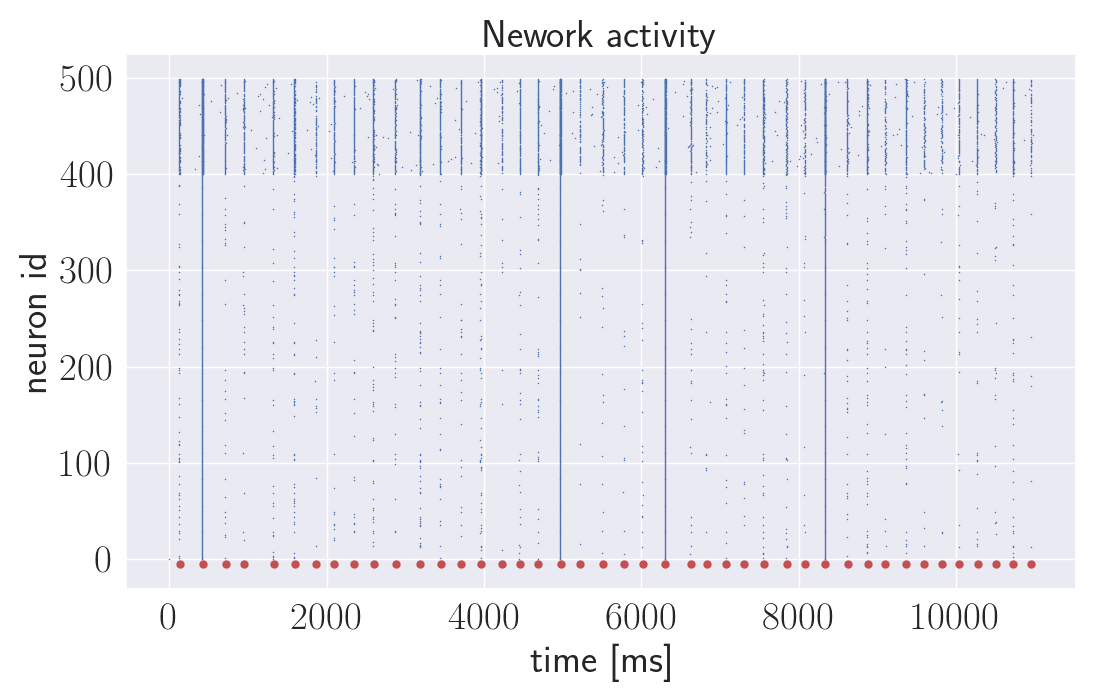
\includegraphics[width=1\textwidth]{images/network.png}
    \caption{\textbf{Reference network activity} The upper fifth are inhibitory neurons, the lower
        four fifths are excitatory ones. Each blue dot is a neuron spiking, and the red dots signify
        Detected network bursts. A bursts is defined as an interval of time where at least ten neurons
        fire within five ms of each other.}
    \label{fig:network-activity}
\end{figure}

% TODO: Neet to make this a subplot
\begin{figure}
    \centering
    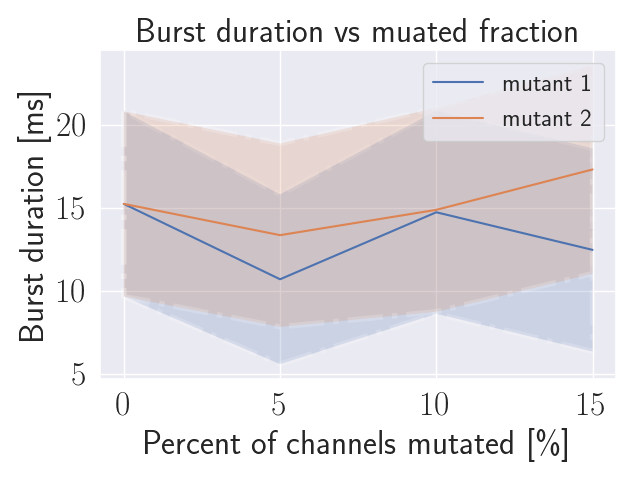
\includegraphics[width=1\textwidth]{images/duration.png}
    \caption{\textbf{The duration of network bursts versus the fraction of mutated sodium channels}
        The error bars are computed across all the network bursts and for three different random
        seeds.}
    \label{fig:duration}
\end{figure}

\begin{figure}
    \centering
    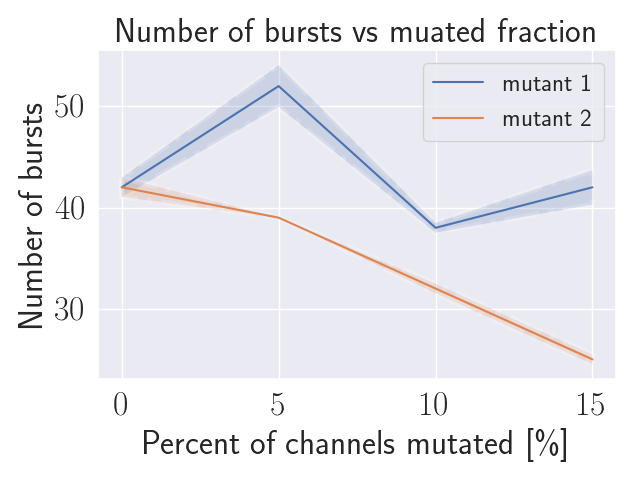
\includegraphics[width=1\textwidth]{images/number.png}
    \caption{\textbf{Number of network bursts versus the fraction of mutated sodium channels} The
        error bars are computed across three random seeds.}
    \label{fig:number}
\end{figure}
